\documentclass[11pt]{article}

\usepackage[T1]{fontenc}
\usepackage[utf8]{inputenc}
\usepackage{lmodern}
\usepackage[a4paper,margin=27mm]{geometry}
\usepackage{microtype}
\usepackage{amsmath,amssymb,amsthm,mathtools,mathrsfs}
% Canonical mathematical notation for active FabiusFunction LaTeX documents.
%
% This file is intentionally a plain TeX input rather than a LaTeX package.
% Every standalone document loads it by an explicit path relative to that
% document's directory; included fragments inherit the definitions from their
% root document.  Keep this file independent of document layout and metadata.
%
% Contract:
%   * one command has one mathematical meaning throughout the active corpus;
%   * names encode semantic roles rather than a document-local choice of letter;
%   * visually similar but differently normalized objects have different print;
%   * every command below is defined normatively in the notation catalogue.
%
% The active corpus excludes docs/archive/.  Historical sources may retain
% their original notation only inside an explicitly labelled quotation.

\makeatletter
\@ifundefined{mathbb}{%
  \PackageError{fabius-notation}{The amssymb package must be loaded first}%
    {Load amsmath and amssymb before inputting fabius-notation.tex.}%
}{}
\@ifundefined{operatorname}{%
  \PackageError{fabius-notation}{The amsmath package must be loaded first}%
    {Load amsmath before inputting fabius-notation.tex.}%
}{}
\makeatother

% Version stamp used by the catalogue and by static audits.
\newcommand{\FabiusNotationVersion}{2026-08-31}

% Number systems.  NaturalNumbers is explicitly the nonnegative convention.
\newcommand{\NaturalNumbers}{\mathbb{N}_{0}}
\newcommand{\PositiveIntegers}{\mathbb{N}_{>0}}
\newcommand{\IntegerNumbers}{\mathbb{Z}}
\newcommand{\RationalNumbers}{\mathbb{Q}}
\newcommand{\RealNumbers}{\mathbb{R}}
\newcommand{\ComplexNumbers}{\mathbb{C}}
\newcommand{\ExtendedRealNumbers}{\overline{\mathbb{R}}}

% The three principal Fabius--Rvachev functions.  Subscripts are deliberate:
% a bare F and a calligraphic F have several unrelated uses in the corpus.
\newcommand{\FabiusBounded}{F_{\mathrm{bd}}}
\newcommand{\FabiusGlobal}{F_{\mathrm{gl}}}
\newcommand{\FabiusQuantile}{Q_{F}}
\newcommand{\FabiusClampedQuantile}{Q_{F,\mathrm{cl}}}
\newcommand{\RvachevUp}{\operatorname{up}}

% Constants, elementary operators, and delimiters.
\newcommand{\EulerE}{\mathrm{e}}
\newcommand{\ImaginaryUnit}{\mathrm{i}}
\newcommand{\Differential}{\mathop{}\!\mathrm{d}}
\newcommand{\AbsoluteValue}[1]{\left\lvert #1\right\rvert}
\newcommand{\Norm}[1]{\left\lVert #1\right\rVert}
\newcommand{\Floor}[1]{\left\lfloor #1\right\rfloor}
\newcommand{\Ceiling}[1]{\left\lceil #1\right\rceil}
\newcommand{\FractionalPart}[1]{\left\{#1\right\}}
\newcommand{\PositivePart}[1]{\left(#1\right)_{+}}
\newcommand{\IndicatorOf}[1]{\mathbf{1}_{#1}}
\newcommand{\SetOf}[1]{\left\{#1\right\}}
\newcommand{\InnerProduct}[1]{\left\langle #1\right\rangle}
\newcommand{\CardinalityOf}[1]{\left\lvert #1\right\rvert}
\newcommand{\DefinitionEquals}{\mathrel{\coloneqq}}
\newcommand{\Sign}{\operatorname{sgn}}
\newcommand{\IdentityOperator}{\operatorname{id}}
\newcommand{\SpanOperator}{\operatorname{span}}
\newcommand{\TraceOperator}{\operatorname{tr}}
\newcommand{\RankOperator}{\operatorname{rank}}
\newcommand{\DiagonalOperator}{\operatorname{diag}}
\newcommand{\ResidueOperator}{\operatorname*{Res}}
\newcommand{\LeastCommonMultiple}{\operatorname{lcm}}
\newcommand{\OrderOperator}{\operatorname{ord}}
\newcommand{\PrincipalLogarithm}{\operatorname{Log}}
\newcommand{\FallingFactorial}[2]{\left(#1\right)^{\underline{#2}}}
\newcommand{\RisingFactorial}[2]{\left(#1\right)^{\overline{#2}}}

% Support, topology, convolution, and metric notation.
\newcommand{\SupportOperator}{\operatorname{supp}}
\newcommand{\SupportOf}[1]{\SupportOperator\!\left(#1\right)}
\newcommand{\TopologicalSupportOf}[1]{\operatorname{tsupp}\!\left(#1\right)}
\newcommand{\Convolution}{\mathbin{*}}
\newcommand{\MetricDistance}{\operatorname{dist}}
\newcommand{\TotalVariationDistance}{d_{\mathrm{TV}}}

% Probability.  Equality and convergence in law are not metric distance.
\newcommand{\Probability}{\mathbb{P}}
\newcommand{\Expectation}{\mathbb{E}}
\newcommand{\Variance}{\operatorname{Var}}
\newcommand{\Covariance}{\operatorname{Cov}}
\newcommand{\LawOperator}{\operatorname{Law}}
\newcommand{\LawOf}[1]{\LawOperator\!\left(#1\right)}
\newcommand{\EqualInLaw}{\mathrel{\overset{\mathrm{law}}{=}}}
\newcommand{\ConvergesInLaw}{\mathrel{\xrightarrow{\mathrm{law}}}}

% Fourier and integral transforms.  The printed labels expose normalization.
% FourierTwoPi uses exp(-2*pi*i*x*xi); FourierAngular uses exp(-i*x*omega).
\newcommand{\FourierTwoPi}[1]{\widehat{#1}_{\,2\pi}}
\newcommand{\FourierAngular}[1]{\widehat{#1}_{\,\mathrm{ang}}}
\newcommand{\LaplaceTransformSymbol}{\mathcal{L}}
\newcommand{\MellinTransformSymbol}{\mathcal{M}}
\newcommand{\LaplaceTransformOf}[1]{\LaplaceTransformSymbol\!\left[#1\right]}
\newcommand{\MellinTransformOf}[1]{\MellinTransformSymbol\!\left[#1\right]}
\newcommand{\MomentGeneratingFunction}[1]{M_{#1}}
\newcommand{\CharacteristicFunction}[1]{\varphi_{#1}}

% The two standard sinc functions must never share one symbol.
\newcommand{\SincRad}{\operatorname{sinc}_{\mathrm{rad}}}
\newcommand{\SincPi}{\operatorname{sinc}_{\pi}}

% Binary arithmetic and Thue--Morse notation.
\newcommand{\BinaryDigitSum}{\operatorname{wt}_{2}}
\newcommand{\ThueMorseSignSymbol}{\varepsilon}
\newcommand{\ThueMorseSign}[1]{\varepsilon_{#1}}
\newcommand{\PadicValuation}[1]{\nu_{#1}}
\newcommand{\TwoAdicValuation}{\nu_{2}}

% q-series notation.  Every base is an explicit argument.
\newcommand{\QPochhammer}[3]{\left(#1;#2\right)_{#3}}
\newcommand{\GaussianBinomial}[3]{%
  \genfrac{[}{]}{0pt}{}{#1}{#2}_{#3}%
}
\newcommand{\QInteger}[2]{\left[#1\right]_{#2}}

% Named special functions.
\newcommand{\Polylogarithm}{\operatorname{Li}}
\newcommand{\LambertW}{W}
\newcommand{\GammaFunction}{\Gamma}
\newcommand{\RiemannZeta}{\zeta}

% Asymptotics.  BigO and LittleO are operator tokens for existing formula
% grammar; prefer the At forms so that the limiting regime is printed.
\newcommand{\BigO}{\mathcal{O}}
\newcommand{\LittleO}{o}
\newcommand{\BigOAt}[2]{\mathcal{O}_{#2}\!\left(#1\right)}
\newcommand{\LittleOAt}[2]{o_{#2}\!\left(#1\right)}

\usepackage{bm}
\usepackage{booktabs,longtable,tabularx,array}
\usepackage{graphicx}
\usepackage{xcolor}
\usepackage{enumitem}
\usepackage{listings}
\usepackage{url}
\usepackage{hyperref}
\usepackage[nameinlink,noabbrev]{cleveref}
\usepackage{fancyhdr}
\usepackage{caption}
\usepackage{subcaption}
\usepackage{float}

\graphicspath{{figures/}}
\hypersetup{
  colorlinks=true,
  linkcolor=blue!45!black,
  citecolor=green!35!black,
  urlcolor=blue!55!black,
  pdftitle={Cyclotomic Blow-Ups and Natural Boundaries for the q-Fabius--Rvachev Sinc Product},
  pdfauthor={Research report for the ProveIt FabiusFunction project}
}

\pagestyle{fancy}
\fancyhf{}
\fancyhead[L]{Cyclotomic $q$-Fabius--Rvachev frontiers}
\fancyhead[R]{\thepage}
\setlength{\headheight}{14pt}

\newtheorem{theorem}{Theorem}[section]
\newtheorem{proposition}[theorem]{Proposition}
\newtheorem{lemma}[theorem]{Lemma}
\newtheorem{corollary}[theorem]{Corollary}
\newtheorem{conjecture}[theorem]{Conjecture}
\newtheorem{problem}[theorem]{Problem}
\theoremstyle{definition}
\newtheorem{definition}[theorem]{Definition}
\newtheorem{example}[theorem]{Example}
\newtheorem{remark}[theorem]{Remark}
\newtheorem{status}[theorem]{Status note}

\DeclareMathOperator{\ord}{ord}
\DeclareMathOperator{\dist}{dist}
\newcommand{\D}{\mathbb D}
\newcommand{\eps}{\varepsilon}
\newcommand{\om}{\omega}
\newcommand{\PhiQ}{\Phi}
\newcommand{\Aact}{\mathscr A}
\newcommand{\Bact}{\mathscr B}
\newcommand{\brak}[1]{\left[#1\right]}
\newcommand{\paren}[1]{\left(#1\right)}
\newcommand{\coeff}[2]{\brak{#1^{#2}}}

\crefname{equation}{equation}{equations}
\Crefname{equation}{Equation}{Equations}

\lstdefinestyle{py}{
  language=Python,
  basicstyle=\ttfamily\small,
  keywordstyle=\color{blue!55!black},
  commentstyle=\color{green!35!black},
  stringstyle=\color{red!45!black},
  breaklines=true,
  frame=single,
  columns=fullflexible,
  showstringspaces=false
}

\title{\bfseries Cyclotomic Blow-Ups and Natural Boundaries\\[4pt]
for the $q$-Fabius--Rvachev Sinc Product\\[8pt]
\large Spectral dilogarithms, polyharmonic limits, Bell condensation, and inverse branches}
\author{Research report for the \texttt{ProveIt/Analysis/FabiusFunction} project}
\date{30 August 2026}

\begin{document}
\maketitle

\begin{abstract}
The dyadic Rvachev up-function has Fourier transform
\(
 \prod_{j\ge 1}\SincRad(z/2^j)
\), and the surrounding repository develops its Fabius, Thue--Morse, $q$-series, Bell--Bernoulli, inverse, sampling, and Lambert-$W$ structures in considerable depth.  The current consolidated $q$-series frontier explicitly leaves two related tasks open: proving a generic natural boundary in the $q$-plane and constructing root-of-unity renormalizations.  This report resolves a concrete scalar version of both tasks for the complex geometric-uniform transform
\[
 \Phi(q,z)=\prod_{j\ge0}\SincRad\bigl((1-q)q^jz\bigr),\qquad |q|<1.
\]

For a primitive $m$th root of unity $\omega$ and
\(d=\ord(\omega^2)=m/\gcd(m,2)\), we derive the radial expansion
\[
 \log\Phi(\omega(1-\delta),z)
 =-\frac{\mathscr A_\omega(z)}{\delta}+\mathscr B_\omega(z)+O(\delta),
\]
locally uniformly for $|(1-\omega)z|<\pi$.  The action is an explicit spectral dilogarithm,
\[
 \mathscr A_\omega(z)=\frac1{2d^2}
 \sum_{n\ge1}\Polylogarithm_2\!\left(\left(\frac{(1-\omega)z}{\pi n}\right)^{2d}\right).
\]
Its sign is never zero for real $0<|z|<\pi/2$.  Because roots of unity are dense, this proves that the unit circle is a natural boundary for $q\mapsto\Phi(q,z)$ throughout that entire frequency interval, strengthening the repository's generic conjecture to an explicit theorem.

A double scaling
\(q=\omega(1-\varepsilon^d)\), \(z=\sqrt\varepsilon\,w\)
then gives the locally uniform cyclotomic limit
\[
 \Phi\bigl(\omega(1-\varepsilon^d),\sqrt\varepsilon\,w\bigr)
 \longrightarrow \exp(-A_\omega w^{2d}),
 \qquad
 A_\omega=\frac{\zeta(2d)(1-\omega)^{2d}}{2d^2\pi^{2d}}.
\]
We prove the first corrections and an all-orders Bell-polynomial expansion, identify the corresponding polyharmonic heat symbol, show that the reciprocal zero moments and Bernoulli cumulants collapse to a single order $2d$, derive the limiting Gould--Hopper Appell family, and construct inverse branches both in the scaled frequency and in $q$ itself.  A universal analytic-germ theorem shows that the mechanism extends beyond sinc products to $q$-Pochhammer and other geometric products.  High-precision experiments, source code, CSV data, and figures accompany the report.
\end{abstract}

\tableofcontents
\clearpage

\section{Scope, status, and contribution boundary}

\subsection{The audited source landscape}

The requested source tree is a living research corpus rather than a single paper.  Its current top level contains the primary Fabius--Rvachev exposition, a mathematical glossary, a non-elementarity study, a Lean walkthrough, imported papers, an archive, and a semi-formalized frontier system.  During August 2026 many formerly separate frontier drafts were consolidated into thematic volumes.  Consequently, a novelty audit based only on old filenames would be misleading: the correct comparison target is the current consolidated mathematics, supplemented by historical inventories for paths that were absorbed or archived.

The audit used three layers.
\begin{enumerate}[label=\arabic*.]
\item The current public GitHub tree, the current semi-formalized README, and the raw consolidated \emph{Exponents and $q$-Series Frontiers} source were inspected at theorem and open-problem level.
\item A preserved recursive ledger of every \texttt{*.tex} path under \texttt{Analysis/FabiusFunction/docs} at commit
\texttt{24da985eba70e46d862acdaddd476793a428213e} was used to retain coverage of the frozen archive and earlier source-paper layout.  The 57-path ledger is included in the companion archive as
\texttt{corpus\_inventory\_2026-08-27.txt}.
\item Prior frontier reports in the user's library were phrase- and formula-searched for the proposed concepts.  In particular, Stein--Koopman calculus, transfer determinants, fractional transforms, dyadic-comb interpolation, inverse-Lambert expansions, Appell deconvolution, and spectral zero-divisor theory were treated as occupied territory and are not presented here as new.
\end{enumerate}

The current consolidated $q$-series volume formulates a \emph{generic natural-boundary conjecture} for its geometric characteristic function and separately asks for \emph{root-of-unity renormalization}.  The present report targets precisely that remaining scalar analytic gap.  It does not claim to solve the full two-nome finite-law, matrix Mahler, or mixed Prouhet problem.

\begin{status}[Meaning of ``new'']
Throughout this report, \emph{new} means apparently new relative to the audited repository corpus.  It is not a claim of worldwide priority.  Classical ingredients such as Euler's sine product, Bernoulli cumulants, $q$-Pochhammer notation, and radial root-of-unity methods are cited and clearly separated from the deductions made here.
\end{status}

\subsection{Result ledger}

The principal contributions are as follows.
\begin{enumerate}[label=\textbf{R\arabic*.},leftmargin=3.4em]
\item An exact logarithmic and $q$-Pochhammer representation of the complex geometric sinc product, organized so that cyclotomic resonance is visible coefficient by coefficient.
\item A two-term radial expansion at every nontrivial root of unity, with an explicit action $\mathscr A_\omega$ and constant term $\mathscr B_\omega$.
\item Three equivalent descriptions of $\mathscr A_\omega$: a resonant zeta series, an infinite spectral dilogarithm, and a cyclic projection integral.
\item A sign theorem for the action and, as a consequence, a proof that the unit circle is a natural boundary for every fixed real $0<|z|<\pi/2$.
\item A root-of-unity blow-up limit to $\exp(-A_\omega w^{2d})$, including subcritical corrections, the complete order-$\varepsilon^d$ layer, and an all-orders Bell-polynomial scheme.
\item A universal analytic-germ theorem that recovers both the sinc result and a root-scaled $q$-Pochhammer limit.
\item Spectral condensation: among all reciprocal zero power sums, exactly the $2d$th survives after cyclotomic scaling.
\item Bernoulli--Bell condensation: among all scaled cumulants, exactly the $2d$th survives, forcing an explicit sparse moment sequence.
\item A limiting Gould--Hopper/Appell family obtained from the inverse moment generating function.
\item Polyharmonic heat-kernel and Stokes-sector interpretations, distinguishing the genuinely dissipative roots $m\equiv2\pmod4$ from backward/rotated sectors.
\item Analytic inverse branches in the scaled frequency and in $q$, with explicit first corrections and predicted monodromy.
\item Reproducible high-precision tests whose fitted convergence exponents agree with the proved orders.
\end{enumerate}

\section{The Fabius--Rvachev interface and its complex $q$-extension}

\subsection{The dyadic probability law}

Let $V_0,V_1,\dots$ be independent random variables uniformly distributed on $[-1,1]$.  The centered dyadic random series
\begin{equation}
 Y_{1/2}=\sum_{j\ge0}2^{-(j+1)}V_j
 \label{eq:dyadic-series}
\end{equation}
has support $[-1,1]$ and density Rvachev's up-function $\RvachevUp$.  Its characteristic function, with the convention $\SincRad z=\sin z/z$, is
\begin{equation}
 \widehat{\RvachevUp}(z)
 =\prod_{j\ge0}\SincRad\!\left(\frac{z}{2^{j+1}}\right).
 \label{eq:up-transform}
\end{equation}
The Fabius distribution on $[0,1]$ is obtained by the affine change
\(X=(Y_{1/2}+1)/2\).  The repository develops this bridge, exact dyadic arithmetic, Thue--Morse derivative signs, moment and cumulant formulas, Legendre expansions, inverse asymptotics, and many related representations.  We use those structures only as motivation and normalization.

\subsection{The geometric family}

For real $0<q<1$, define
\begin{equation}
 Y_q=(1-q)\sum_{j\ge0}q^jV_j.
 \label{eq:Yq}
\end{equation}
The coefficient sum is one, so $Y_q$ is again supported on $[-1,1]$.  Independence gives
\begin{equation}
 \mathbb E\EulerE^{\ImaginaryUnit zY_q}
 =\prod_{j\ge0}\SincRad\bigl((1-q)q^jz\bigr).
 \label{eq:real-char}
\end{equation}
For complex $q$ there is generally no positive probability law, but the product itself remains a natural analytic object.

\begin{definition}[Complex $q$-Fabius--Rvachev sinc product]
For $q\in\D=\SetOf{q\in\ComplexNumbers:|q|<1}$ and $z\in\ComplexNumbers$, set
\begin{equation}
 \Phi(q,z)=\prod_{j=0}^{\infty}
 \SincRad\bigl((1-q)q^jz\bigr).
 \label{eq:Phi-def}
\end{equation}
\end{definition}

\begin{proposition}[Holomorphy and normalization]
The product in \cref{eq:Phi-def} converges locally uniformly on $\D\times\ComplexNumbers$ and defines a holomorphic function there.  Moreover,
\[
 \Phi(q,0)=1,
 \qquad
 \Phi(0,z)=\SincRad z,
 \qquad
 \Phi\left(\tfrac12,z\right)=\widehat{\RvachevUp}(z).
\]
\end{proposition}

\begin{proof}
On a compact set $|q|\le r<1$, $|z|\le R$, the $j$th argument is $O(r^j)$ uniformly.  Since $\SincRad w=1-w^2/6+O(w^4)$, the deviation of the $j$th factor from one is $O(r^{2j})$.  The Weierstrass criterion gives locally uniform convergence of the product and of its holomorphic finite approximants.  The three normalizations follow directly.
\end{proof}

\section{Master logarithmic and $q$-Pochhammer representations}

\subsection{The exact logarithmic series}

Euler's sine product and its logarithm give
\begin{equation}
 \SincRad w=\prod_{n\ge1}\left(1-\frac{w^2}{\pi^2n^2}\right),
 \qquad
 \log\SincRad w=-\sum_{k\ge1}c_kw^{2k},
 \label{eq:sinc-log}
\end{equation}
where
\begin{equation}
 c_k=\frac{\zeta(2k)}{k\pi^{2k}}>0.
 \label{eq:ck}
\end{equation}
The logarithm is the branch normalized by $\log\SincRad0=0$ in $|w|<\pi$.

\begin{theorem}[Master logarithm]
On the domain
\[
 \Omega=\SetOf{(q,z)\in\D\times\ComplexNumbers: |(1-q)z|<\pi},
\]
one has the absolutely and locally uniformly convergent expansion
\begin{equation}
 \boxed{
 \log\Phi(q,z)
 =-\sum_{k\ge1}c_k
 \frac{(1-q)^{2k}}{1-q^{2k}}z^{2k}.}
 \label{eq:master-log}
\end{equation}
\end{theorem}

\begin{proof}
For $(q,z)\in\Omega$, every argument $(1-q)q^jz$ lies in the zero-free disk $|w|<\pi$.  Insert \cref{eq:sinc-log}, sum first over $j$, and use
\(
 \sum_{j\ge0}q^{2kj}=(1-q^{2k})^{-1}
\).  Absolute local uniformity follows from a geometric majorant because
\(
 c_k\le C\pi^{-2k}/k
\)
and $|(1-q)z|$ stays below $\pi$ on compact subsets.
\end{proof}

The coefficient
\begin{equation}
 R_k(q):=\frac{(1-q)^{2k}}{1-q^{2k}}
 \label{eq:Rk}
\end{equation}
is simultaneously a geometric power sum, a cumulant multiplier, and the source of every root-of-unity singularity.  The entire cyclotomic theory below is a careful organization of the resonances $q^{2k}=1$.

\subsection{A spectral $q$-Pochhammer factorization}

Let $(a;Q)_\infty=\prod_{j\ge0}(1-aQ^j)$.  Reordering Euler's sine factors gives a second exact representation.

\begin{theorem}[Infinite spectral $q$-Pochhammer product]
For every $q\in\D$ and $z\in\ComplexNumbers$,
\begin{equation}
 \boxed{
 \Phi(q,z)=\prod_{n\ge1}
 \left(\frac{(1-q)^2z^2}{\pi^2n^2};q^2\right)_\infty.}
 \label{eq:qpoch-factor}
\end{equation}
The double product is locally normally convergent.
\end{theorem}

\begin{proof}
Apply Euler's product to each sinc factor:
\[
 \prod_{j\ge0}\prod_{n\ge1}
 \left(1-\frac{(1-q)^2q^{2j}z^2}{\pi^2n^2}\right).
\]
The sum of absolute first-order deviations is bounded on compact sets by a constant multiple of
\(
 \sum_j|q|^{2j}\sum_nn^{-2}<\infty
\), so the products may be interchanged.  The inner product over $j$ is the stated $q^2$-Pochhammer symbol.
\end{proof}

\begin{remark}[Why dilogarithms appear]
Radial root-of-unity asymptotics of a single $q$-Pochhammer symbol are governed by a dilogarithmic action and a finite cyclic factor.  Formula \cref{eq:qpoch-factor} superposes one such action for each spectral point $\pi n$.  The result is the infinite spectral dilogarithm obtained below.  Our direct proof from \cref{eq:master-log} avoids branch bookkeeping and makes the uniformity transparent.
\end{remark}

\section{Radial resonance at roots of unity}

\subsection{Cyclotomic notation}

Fix a primitive $m$th root
\begin{equation}
 \omega=\exp\left(\frac{2\pi\ImaginaryUnit h}{m}\right),
 \qquad (h,m)=1,
 \qquad m\ge2,
 \label{eq:omega}
\end{equation}
and write
\begin{equation}
 d=\ord(\omega^2)=\frac{m}{\gcd(m,2)},
 \qquad
 a_\omega=1-\omega.
 \label{eq:d-a}
\end{equation}
Thus $\omega^{2k}=1$ exactly when $d\mid k$.  We approach the root radially from inside the disk by
\begin{equation}
 q=\omega(1-\delta),
 \qquad \delta\downarrow0.
 \label{eq:radial-q}
\end{equation}

\begin{lemma}[Resonant and nonresonant multipliers]
For fixed $k\ge1$,
\begin{align}
 \frac{(1-q)^{2k}}{1-q^{2k}}
 &=\frac{a_\omega^{2k}}{1-\omega^{2k}}+O(\delta),
 && d\nmid k,
 \label{eq:nonres-exp}\\[3pt]
 \frac{(1-q)^{2k}}{1-q^{2k}}
 &=a_\omega^{2k}\left[
 \frac{1}{2k\delta}
 +\frac{\omega}{1-\omega}
 +\frac{2k-1}{4k}
 +O(\delta)
 \right],
 && d\mid k.
 \label{eq:res-exp}
\end{align}
The error is uniform for $k$ in any fixed residue class, after multiplication by a geometrically decaying factor $\rho^{2k}$ with $0<\rho<1$.
\end{lemma}

\begin{proof}
The nonresonant denominator tends to the nonzero number $1-\omega^{2k}$.  In the resonant case,
\begin{align*}
 (1-q)^{2k}
 &=a_\omega^{2k}
 \left(1+2k\frac{\omega}{a_\omega}\delta+O(k^2\delta^2)\right),\\
 1-q^{2k}
 &=1-(1-\delta)^{2k}
 =2k\delta-k(2k-1)\delta^2+O(k^3\delta^3).
\end{align*}
Divide the two expansions.  The final uniformity statement follows because the Taylor coefficients grow at most polynomially in $k$.
\end{proof}

\subsection{The radial action and constant term}

\begin{definition}[Cyclotomic action]
For $|a_\omega z|<\pi$, define
\begin{equation}
 \Aact_\omega(z)
 =\sum_{\ell\ge1}
 \frac{c_{\ell d}}{2\ell d}
 a_\omega^{2\ell d}z^{2\ell d}.
 \label{eq:action-series}
\end{equation}
Also define
\begin{align}
 \Bact_\omega(z)
 =&-\sum_{\substack{k\ge1\\d\nmid k}}
 c_k\frac{a_\omega^{2k}}{1-\omega^{2k}}z^{2k}
 \label{eq:B-first}\\
 &-\sum_{\substack{k\ge1\\d\mid k}}
 c_ka_\omega^{2k}
 \left(\frac{\omega}{1-\omega}+\frac{2k-1}{4k}\right)z^{2k}.
 \label{eq:B-second}
\end{align}
\end{definition}

\begin{theorem}[Two-term radial root-of-unity expansion]
Let $K$ be a compact subset of $\SetOf{z:|a_\omega z|<\pi}$.  Uniformly for $z\in K$,
\begin{equation}
 \boxed{
 \log\Phi\bigl(\omega(1-\delta),z\bigr)
 =-\frac{\Aact_\omega(z)}{\delta}
 +\Bact_\omega(z)+O_K(\delta).}
 \label{eq:two-term-radial}
\end{equation}
In particular, every nontrivial root of unity carries a full exponential-scale singularity unless $\Aact_\omega(z)=0$.
\end{theorem}

\begin{proof}
Insert \cref{eq:nonres-exp,eq:res-exp} into \cref{eq:master-log}.  The coefficients of $\delta^{-1}$ are exactly the resonant terms $k=\ell d$ and sum to $-\Aact_\omega(z)/\delta$.  The constant terms are \cref{eq:B-first,eq:B-second}.  Choose $\rho<1$ with $|a_\omega z|\le\rho\pi$ on $K$.  Since $c_k|a_\omega z|^{2k}=O(\rho^{2k}/k)$ and the expansion remainders have at most polynomial growth in $k$, their sum is $O_K(\delta)$.
\end{proof}

\subsection{Dilogarithmic and cyclic descriptions}

The action has two additional forms that expose its spectral and finite-cyclic content.

\begin{theorem}[Spectral dilogarithm]
For $|a_\omega z|<\pi$,
\begin{equation}
 \boxed{
 \Aact_\omega(z)
 =\frac{1}{2d^2}\sum_{n\ge1}
 \Polylogarithm_2\!\left(
 \left(\frac{a_\omega z}{\pi n}\right)^{2d}
 \right).}
 \label{eq:spectral-dilog}
\end{equation}
The series converges absolutely and locally uniformly.
\end{theorem}

\begin{proof}
Expand $\zeta(2\ell d)=\sum_{n\ge1}n^{-2\ell d}$ in \cref{eq:action-series}, then interchange the absolutely convergent sums:
\begin{align*}
 \Aact_\omega(z)
 &=\sum_{n\ge1}\sum_{\ell\ge1}
 \frac1{2(\ell d)^2}
 \left(\frac{a_\omega z}{\pi n}\right)^{2\ell d}\\
 &=\frac1{2d^2}\sum_{n\ge1}
 \Polylogarithm_2\!\left(\left(\frac{a_\omega z}{\pi n}\right)^{2d}\right).
\end{align*}
\end{proof}

\begin{theorem}[Cyclic projection formula]
For $|a_\omega z|<\pi$,
\begin{equation}
 \boxed{
 \Aact_\omega(z)
 =-\int_0^z
 \left[
 \frac1d\sum_{r=0}^{d-1}
 \log\SincRad(a_\omega\omega^rt)
 \right]\frac{\Differential t}{t}.}
 \label{eq:cyclic-projection}
\end{equation}
The integrand has a removable singularity at zero.
\end{theorem}

\begin{proof}
Average the logarithmic series:
\[
 \frac1d\sum_{r=0}^{d-1}\log\SincRad(a_\omega\omega^rt)
 =-\sum_{k\ge1}c_ka_\omega^{2k}t^{2k}
 \left(\frac1d\sum_{r=0}^{d-1}\omega^{2kr}\right).
\]
The parenthesized average is one if $d\mid k$ and zero otherwise.  Integrating termwise gives \cref{eq:action-series}.
\end{proof}

\begin{remark}
Formula \cref{eq:cyclic-projection} is a root-of-unity filter in the scale index.  The sinc function is even, so the relevant cycle is generated by $\omega^2$, not $\omega$; this explains the compression from order $m$ to $d=m/\gcd(m,2)$.
\end{remark}

\section{A natural-boundary theorem}

\subsection{The sign of the action}

The crucial point is that the action cannot vanish on a uniform real-frequency interval.

\begin{lemma}[Reality and sign of $a_\omega^{2d}$]
The number $a_\omega^{2d}$ is real and nonzero.  For a primitive $m$th root,
\begin{equation}
 \Sign\bigl(a_\omega^{2d}\bigr)=
 \begin{cases}
 -1,&m\text{ odd},\\
 (-1)^{d+1},&m\text{ even}.
 \end{cases}
 \label{eq:sign-a}
\end{equation}
Thus it is positive exactly when $m\equiv2\pmod4$.
\end{lemma}

\begin{proof}
Write $\omega=\EulerE^{\ImaginaryUnit\theta}$.  Since
\(
 1-\EulerE^{\ImaginaryUnit\theta}=-2\ImaginaryUnit\EulerE^{\ImaginaryUnit\theta/2}\sin(\theta/2)
\),
\[
 a_\omega^{2d}=(-4)^d\EulerE^{\ImaginaryUnit d\theta}\sin^{2d}(\theta/2).
\]
If $m$ is odd then $d=m$ and $\EulerE^{\ImaginaryUnit d\theta}=1$, while $d$ is odd.  If $m$ is even then $d=m/2$, the primitive numerator $h$ is odd, and $\EulerE^{\ImaginaryUnit d\theta}=\EulerE^{\ImaginaryUnit\pi h}=-1$.  The signs follow.
\end{proof}

\begin{theorem}[Nonvanishing action on a universal interval]
For every primitive root $\omega\ne1$ and every real $z$ with
\begin{equation}
 0<|z|<\frac\pi2,
 \label{eq:zinterval}
\end{equation}
$\Aact_\omega(z)$ is real, nonzero, and
\begin{equation}
 \Sign\Aact_\omega(z)=\Sign(a_\omega^{2d}).
 \label{eq:sign-action}
\end{equation}
\end{theorem}

\begin{proof}
Because $|a_\omega|\le2$, condition \cref{eq:zinterval} implies
\(
 |a_\omega z/(\pi n)|<1
\) for every $n\ge1$.  By \cref{eq:sign-a},
\[
 \left(\frac{a_\omega z}{\pi n}\right)^{2d}
 =\sigma x_n,
 \qquad
 \sigma\in\SetOf{-1,1},\quad 0<x_n<1.
\]
For $0<x<1$, $\Polylogarithm_2(x)>0$ and $\Polylogarithm_2(-x)<0$.  Every summand in \cref{eq:spectral-dilog} therefore has sign $\sigma$, proving the claim.
\end{proof}

\subsection{Natural boundary}

\begin{theorem}[Explicit natural boundary for the $q$-Fabius sinc transform]
Fix real $z$ with $0<|z|<\pi/2$.  The holomorphic function
\begin{equation}
 q\longmapsto\Phi(q,z),\qquad |q|<1,
 \label{eq:qmap}
\end{equation}
has the unit circle as a natural boundary.  More strongly, it admits no single-valued meromorphic continuation through any nontrivial boundary arc.
\end{theorem}

\begin{proof}
Let $\omega\ne1$ be any root of unity.  By the preceding theorem,
\(
 A:=\Aact_\omega(z)\in\RealNumbers\setminus\SetOf0
\).  From \cref{eq:two-term-radial},
\begin{equation}
 \log|\Phi(\omega(1-\delta),z)|
 =-\frac{A}{\delta}+O(1).
 \label{eq:mod-growth}
\end{equation}
If $A>0$, the modulus tends to zero faster than every power of $\delta$.  A holomorphic continuation through $\omega$ would either be nonzero there or have a zero of finite order, both incompatible with this decay.  A zero of infinite order would force the continuation to vanish identically near $\omega$, hence everywhere in the connected disk by identity, contradicting $\Phi(0,z)=\SincRad z\ne0$.

If $A<0$, the modulus grows faster than every power of $\delta$.  This is incompatible not only with a holomorphic continuation but also with a meromorphic continuation, whose singularity could have only finite pole order.

Thus every nontrivial root of unity is a nonmeromorphic boundary singularity.  Roots of unity are dense on $|q|=1$, so no open boundary arc can be crossed.
\end{proof}

\begin{remark}[What has and has not been proved]
The theorem settles the repository's natural-boundary conjecture for the explicit, nonempty, root-independent interval $0<|z|<\pi/2$.  It does not yet classify exceptional complex frequencies outside that interval.  There the action can cross dilogarithm branch cuts, and cancellation between spectral terms is a genuine possibility.
\end{remark}

\section{Cyclotomic blow-ups}

The fixed-frequency expansion diverges like $\delta^{-1}$.  A nontrivial local limit appears when the frequency shrinks at the exact resonant rate.

\subsection{Leading blow-up theorem}

Set
\begin{equation}
 q_\eps=\omega(1-\eps^d),
 \qquad
 z=\sqrt\eps\,w,
 \qquad \eps\downarrow0,
 \label{eq:blowup-scaling}
\end{equation}
and define
\begin{equation}
 A_\omega
 =\frac{c_d a_\omega^{2d}}{2d}
 =\frac{\zeta(2d)a_\omega^{2d}}{2d^2\pi^{2d}}.
 \label{eq:Aomega}
\end{equation}

\begin{theorem}[Cyclotomic blow-up limit]
Locally uniformly for $w\in\ComplexNumbers$,
\begin{equation}
 \boxed{
 \Phi(q_\eps,\sqrt\eps\,w)
 \longrightarrow \exp(-A_\omega w^{2d}).}
 \label{eq:blowup-limit}
\end{equation}
\end{theorem}

\begin{proof}
In \cref{eq:master-log}, the $k$th term acquires the factor $\eps^k$.  If $d\nmid k$, the multiplier \cref{eq:Rk} remains bounded and the term tends to zero.  If $k=\ell d$, its multiplier is asymptotic to
\(
 a_\omega^{2k}/(2k\eps^d)
\), so the term has order $\eps^{(\ell-1)d}$.  Only $k=d$ survives, giving $-A_\omega w^{2d}$.  On compact $w$-sets, the remaining terms are dominated by a convergent geometric series, which proves local uniformity and permits exponentiation.
\end{proof}

\subsection{Subcritical and order-$d$ corrections}

For $1\le k<d$ define
\begin{equation}
 C_{k,\omega}
 =c_k\frac{a_\omega^{2k}}{1-\omega^{2k}},
 \label{eq:Ck}
\end{equation}
and set
\begin{equation}
 \eta_\omega=\frac{2d\omega}{1-\omega}+\frac{2d-1}{2},
 \qquad
 D_\omega=\frac{c_{2d}a_\omega^{4d}}{4d}.
 \label{eq:eta-D}
\end{equation}

\begin{theorem}[First complete correction layers]
Uniformly on compact $w$-sets,
\begin{align}
 \log\Phi(q_\eps,\sqrt\eps\,w)
 =&-A_\omega w^{2d}
 -\sum_{k=1}^{d-1}C_{k,\omega}\eps^kw^{2k}
 \label{eq:correction-1}\\
 &-\eps^d\left(
 A_\omega\eta_\omega w^{2d}
 +D_\omega w^{4d}
 \right)
 +O(\eps^{d+1}).
 \label{eq:correction-2}
\end{align}
\end{theorem}

\begin{proof}
For $k<d$ there is no resonance, so the constant term of the multiplier gives \cref{eq:Ck}.  At total order $\eps^d$, two and only two resonant sources contribute.  The next term in the $k=d$ multiplier is the constant in \cref{eq:res-exp}, producing $A_\omega\eta_\omega w^{2d}$.  The leading pole of the $k=2d$ multiplier produces $D_\omega w^{4d}$.  Every omitted nonresonant term begins at $k=d+1$, and every later resonant term begins at order at least $2d$, so the remainder is $O(\eps^{d+1})$.
\end{proof}

\subsection{All orders and Bell polynomials}

Define the Laurent germ
\begin{equation}
 \mathcal R_k(\eps)
 =\frac{(a_\omega+\omega\eps^d)^{2k}}
 {1-\omega^{2k}(1-\eps^d)^{2k}}.
 \label{eq:Rkeps}
\end{equation}
For $d\nmid k$ it is analytic at zero; for $d\mid k$ it has a simple pole in $\eps^d$.

\begin{theorem}[All-orders logarithmic expansion]
There are even polynomials $L_n(w)$ such that, as a locally uniform asymptotic expansion,
\begin{equation}
 \log\Phi(q_\eps,\sqrt\eps\,w)
 \sim -A_\omega w^{2d}+\sum_{n\ge1}L_n(w)\eps^n,
 \label{eq:all-log}
\end{equation}
where the coefficient is the finite sum
\begin{equation}
 \boxed{
 L_n(w)=-\sum_{k=1}^{n+d}c_kw^{2k}
 \coeff{\eps}{n-k}\mathcal R_k(\eps).}
 \label{eq:Ln}
\end{equation}
Consequently,
\begin{equation}
 \Phi(q_\eps,\sqrt\eps\,w)
 \sim \EulerE^{-A_\omega w^{2d}}
 \left(1+\sum_{n\ge1}P_n(w)\eps^n\right),
 \label{eq:all-Phi}
\end{equation}
with
\begin{equation}
 \boxed{
 P_n(w)=\frac1{n!}
 B_n\bigl(1!L_1(w),2!L_2(w),\dots,n!L_n(w)\bigr),}
 \label{eq:Bell-Pn}
\end{equation}
where $B_n$ is the complete exponential Bell polynomial.
\end{theorem}

\begin{proof}
Substitute \cref{eq:Rkeps} into the master logarithm.  The coefficient of $\eps^n$ in the $k$th term is the displayed Laurent coefficient with index $n-k$.  Since the lowest possible exponent in $\mathcal R_k$ is $-d$, only $k\le n+d$ can contribute, so the sum is finite.  Truncation with a compact-uniform geometric tail proves the asymptotic statement.  Formula \cref{eq:Bell-Pn} is the standard exponential formula for exponentiating a formal series.
\end{proof}

\begin{remark}
This is a second Bell structure in the theory.  The repository's Bell polynomials encode moments from cumulants; here the same combinatorial transform encodes multiplicative cyclotomic corrections from logarithmic ones.  The two uses meet in \cref{sec:bell-collapse}.
\end{remark}

\subsection{Four small root orders}

\begin{example}[The root $\omega=-1$]
Here $m=2$, $d=1$, and $A_{-1}=1/3$.  Thus
\begin{equation}
 \log\Phi(-1+\eps,\sqrt\eps\,w)
 =-\frac{w^2}{3}
 +\eps\left(\frac{w^2}{6}-\frac{w^4}{45}\right)
 +O(\eps^2).
 \label{eq:m2}
\end{equation}
The first cyclotomic limit is Gaussian.
\end{example}

\begin{example}[Primitive cube root]
For $\omega=\EulerE^{2\pi\ImaginaryUnit/3}$, $d=3$ and $A_\omega=-1/630$.  Moreover
\[
 C_{1,\omega}=-\frac{\ImaginaryUnit}{2\sqrt3},
 \qquad
 C_{2,\omega}=-\frac{\ImaginaryUnit}{20\sqrt3}.
\]
Hence
\begin{equation}
 \log\Phi\bigl(\omega(1-\eps^3),\sqrt\eps\,w\bigr)
 =\frac{w^6}{630}
 +\frac{\ImaginaryUnit\eps w^2}{2\sqrt3}
 +\frac{\ImaginaryUnit\eps^2w^4}{20\sqrt3}
 +O(\eps^3).
 \label{eq:m3}
\end{equation}
The real-axis limit grows, so its transform interpretation belongs to rotated Stokes sectors.
\end{example}

\begin{example}[Fourth root]
For $\omega=\ImaginaryUnit$, $d=2$, $A_\omega=-1/180$, and $C_{1,\omega}=-\ImaginaryUnit/6$.  Therefore
\begin{align}
 \log\Phi\bigl(\ImaginaryUnit(1-\eps^2),\sqrt\eps\,w\bigr)
 =&\frac{w^4}{180}+\frac{\ImaginaryUnit\eps w^2}{6}
 \label{eq:m4-first}\\
 &-\eps^2\left[
 \left(\frac1{360}-\frac{\ImaginaryUnit}{90}\right)w^4
 +\frac{w^8}{18900}
 \right]+O(\eps^3).
 \label{eq:m4-second}
\end{align}
\end{example}

\begin{example}[Primitive sixth root]
For $\omega=\EulerE^{\pi\ImaginaryUnit/3}$, $d=3$, $A_\omega=1/17010$,
\[
 C_{1,\omega}=-\frac{\ImaginaryUnit}{6\sqrt3},
 \qquad
 C_{2,\omega}=\frac{\ImaginaryUnit\sqrt3}{540}.
\]
Thus
\begin{equation}
 \log\Phi\bigl(\omega(1-\eps^3),\sqrt\eps\,w\bigr)
 =-\frac{w^6}{17010}
 +\frac{\ImaginaryUnit\eps w^2}{6\sqrt3}
 -\frac{\ImaginaryUnit\sqrt3\eps^2w^4}{540}
 +O(\eps^3).
 \label{eq:m6}
\end{equation}
This is the first genuinely higher-order dissipative limit.
\end{example}

\section{A universal analytic-germ principle}

The sinc product is one instance of a more general mechanism.

\begin{theorem}[Universal resonant germ]
Let $h$ be analytic near zero, with $h(0)=1$, and choose the local logarithm
\begin{equation}
 \log h(z)=\sum_{n\ge1}b_nz^n.
 \label{eq:germ-log}
\end{equation}
For $|q|<1$ define
\begin{equation}
 \mathcal P_h(q,z)=\prod_{j\ge0}h\bigl((1-q)q^jz\bigr).
 \label{eq:Ph}
\end{equation}
Fix a root $\omega\ne1$, and let
\begin{equation}
 r=\min\SetOf{n\ge1:b_n\ne0\ \text{and}\ \omega^n=1}.
 \label{eq:r-germ}
\end{equation}
Assume this set is nonempty.  Then, locally uniformly for $w$,
\begin{equation}
 \boxed{
 \mathcal P_h\bigl(\omega(1-\delta),\delta^{1/r}w\bigr)
 \longrightarrow
 \exp\left(\frac{b_r(1-\omega)^r}{r}w^r\right).}
 \label{eq:universal-germ}
\end{equation}
\end{theorem}

\begin{proof}
The logarithm of \cref{eq:Ph} is
\[
 \sum_{n\ge1}b_n\frac{(1-q)^n}{1-q^n}z^n.
\]
For nonresonant $n$, the multiplier stays bounded and the scaled term is $O(\delta^{n/r})$.  For resonant $n$, it is asymptotic to $(1-\omega)^n/(n\delta)$, so the scaled order is $\delta^{n/r-1}$.  By the definition of $r$, exactly the $n=r$ term survives.  Compact-uniform convergence follows from the analyticity radius of $h$.
\end{proof}

\begin{corollary}[Sinc and $q$-Pochhammer specializations]
For $h(z)=\SincRad z$, only even coefficients occur and the first resonance is $r=2d$, recovering \cref{eq:blowup-limit}.  For $h(z)=1-z$ and a primitive $m$th root, $r=m$ and
\begin{equation}
 \prod_{j\ge0}
 \left(1-(1-q)q^j\delta^{1/m}w\right)
 \longrightarrow
 \exp\left(-\frac{(1-\omega)^m}{m^2}w^m\right).
 \label{eq:qpoch-germ-limit}
\end{equation}
\end{corollary}

\begin{remark}
The theorem separates three ingredients: the local Taylor support of $\log h$, the cyclic order of $\omega$, and the geometric denominator $1-q^n$.  It therefore applies to many $q$-analog kernels, not merely to the Fabius family.
\end{remark}

\section{Spectral zero condensation}

\subsection{The zero cloud}

Every sinc factor contributes zeros
\begin{equation}
 z_{\ell,j}(q)=\frac{\pi\ell}{(1-q)q^j},
 \qquad \ell\in\IntegerNumbers\setminus\SetOf0,
 \quad j\ge0.
 \label{eq:zeros}
\end{equation}
For positive $\ell$, define the reciprocal even power sum
\begin{equation}
 S_k(q)=\sum_{j\ge0}\sum_{\ell\ge1}z_{\ell,j}(q)^{-2k}.
 \label{eq:Sk-def}
\end{equation}

\begin{proposition}[Exact reciprocal zero moments]
For every $k\ge1$,
\begin{equation}
 \boxed{
 S_k(q)=\frac{\zeta(2k)}{\pi^{2k}}
 \frac{(1-q)^{2k}}{1-q^{2k}}.}
 \label{eq:Sk}
\end{equation}
Moreover, the master logarithm is the canonical zero-moment expansion
\begin{equation}
 \log\Phi(q,z)=-\sum_{k\ge1}\frac{S_k(q)}{k}z^{2k}.
 \label{eq:log-Sk}
\end{equation}
\end{proposition}

\begin{proof}
Insert \cref{eq:zeros}, then separate the geometric and zeta sums.  Formula \cref{eq:log-Sk} is equivalent to \cref{eq:master-log} because $c_k=S_k(q)k^{-1}$ after removing the multiplier.
\end{proof}

\begin{theorem}[One surviving spectral moment]
Under the cyclotomic scaling \cref{eq:blowup-scaling},
\begin{equation}
 \eps^kS_k(q_\eps)\longrightarrow
 \begin{cases}
 \displaystyle
 \frac{\zeta(2d)}{\pi^{2d}}
 \frac{a_\omega^{2d}}{2d},&k=d,\\[7pt]
 0,&k\ne d.
 \end{cases}
 \label{eq:spectral-collapse}
\end{equation}
\end{theorem}

\begin{proof}
If $d\nmid k$, the multiplier in \cref{eq:Sk} remains bounded.  If $k=\ell d$, it grows like $\eps^{-d}$, so multiplication by $\eps^k$ gives $\eps^{(\ell-1)d}$.  Only $\ell=1$ survives.
\end{proof}

\begin{remark}[Escaping zeros leave an exponential trace]
The limiting entire function $\EulerE^{-A_\omega w^{2d}}$ has no zeros.  The zero cloud of the rescaled sinc product escapes to infinity, but its $2d$th reciprocal moment remains finite and becomes the exponential factor in the Hadamard limit.  All other reciprocal moments disappear.
\end{remark}

\section{Bernoulli cumulants, Bell moments, and Appell collapse}
\label{sec:bell-collapse}

\subsection{Complex moment functional}

For real $0<q<1$, the moment generating function of $Y_q$ is
\begin{equation}
 M(q,t)=\mathbb E\EulerE^{tY_q}
 =\Phi(q,\ImaginaryUnit t)
 =\prod_{j\ge0}
 \frac{\sinh((1-q)q^jt)}{(1-q)q^jt}.
 \label{eq:MGF}
\end{equation}
For complex $q$, \cref{eq:MGF} defines an entire generating function and hence a complex moment functional.  The classical Bernoulli expansion gives
\begin{equation}
 \kappa_{2k}(q)
 =\frac{2^{2k-1}B_{2k}}{k}
 \frac{(1-q)^{2k}}{1-q^{2k}},
 \qquad
 \kappa_{2k+1}(q)=0.
 \label{eq:cumulants}
\end{equation}

\begin{theorem}[Cyclotomic cumulant condensation]
Let $Z_\eps=\sqrt\eps\,Y_{q_\eps}$ at the level of formal moments.  Then
\begin{equation}
 \kappa_n(Z_\eps)\longrightarrow0
 \quad(n\ne2d),
 \label{eq:kappa-vanish}
\end{equation}
and
\begin{equation}
 \boxed{
 \kappa_{2d}(Z_\eps)\longrightarrow
 K_{2d,\omega}
 =\frac{2^{2d-2}B_{2d}a_\omega^{2d}}{d^2}.}
 \label{eq:kappa-survive}
\end{equation}
Equivalently, coefficientwise near $t=0$,
\begin{equation}
 M(q_\eps,\sqrt\eps\,t)
 \longrightarrow \exp(B_\omega t^{2d}),
 \qquad
 B_\omega=(-1)^{d+1}A_\omega
 =\frac{K_{2d,\omega}}{(2d)!}.
 \label{eq:MGF-limit}
\end{equation}
\end{theorem}

\begin{proof}
Apply the same resonance count as in \cref{eq:spectral-collapse} to \cref{eq:cumulants}, remembering that scaling by $\sqrt\eps$ multiplies the $n$th cumulant by $\eps^{n/2}$.  The identity between $B_\omega$ and $A_\omega$ follows from Euler's formula for $B_{2d}$ in terms of $\zeta(2d)$.
\end{proof}

\begin{corollary}[Sparse Bell moment limit]
Let $m_n(q)$ be the moments generated by $M(q,t)$.  Then
\begin{equation}
 \eps^{n/2}m_n(q_\eps)\longrightarrow0
 \quad\text{unless }n=2dr,
 \label{eq:mom-zero}
\end{equation}
and for $r\ge0$,
\begin{equation}
 \boxed{
 \eps^{dr}m_{2dr}(q_\eps)
 \longrightarrow
 \frac{(2dr)!}{r!}B_\omega^r.}
 \label{eq:mom-survive}
\end{equation}
\end{corollary}

\begin{proof}
Expand $\exp(B_\omega t^{2d})$.  Equivalently, apply the complete Bell polynomial to a cumulant list with exactly one nonzero entry.
\end{proof}

\subsection{Limiting Appell family}

Let $\mathcal A_n^{(q)}$ denote the inverse-moment Appell polynomials generated by
\begin{equation}
 \frac{\EulerE^{xt}}{M(q,t)}
 =\sum_{n\ge0}\mathcal A_n^{(q)}(x)\frac{t^n}{n!}.
 \label{eq:Appell-q}
\end{equation}
Define the scaled family
\begin{equation}
 \widetilde{\mathcal A}_{n,\eps}(x)
 =\eps^{n/2}\mathcal A_n^{(q_\eps)}(x/\sqrt\eps).
 \label{eq:Appell-scaled}
\end{equation}

\begin{theorem}[Gould--Hopper cyclotomic limit]
Coefficientwise as $\eps\downarrow0$,
\begin{equation}
 \widetilde{\mathcal A}_{n,\eps}(x)
 \longrightarrow H_n^{(d,B_\omega)}(x),
 \label{eq:Appell-limit}
\end{equation}
where
\begin{equation}
 \sum_{n\ge0}H_n^{(d,B)}(x)\frac{t^n}{n!}
 =\EulerE^{xt-Bt^{2d}}
 \label{eq:GH-gen}
\end{equation}
and explicitly
\begin{equation}
 \boxed{
 H_n^{(d,B)}(x)
 =n!\sum_{r=0}^{\Floor{n/(2d)}}
 \frac{(-B)^r x^{n-2dr}}{r!(n-2dr)!}.}
 \label{eq:GH-explicit}
\end{equation}
These polynomials satisfy
\begin{equation}
 H_n^{(d,B)}=\EulerE^{-BD^{2d}}x^n,
 \qquad
 H_{n+1}^{(d,B)}=
 \left(x-2dB D^{2d-1}\right)H_n^{(d,B)},
 \quad D=\frac{\Differential}{\Differential x}.
 \label{eq:GH-operator}
\end{equation}
\end{theorem}

\begin{proof}
The generating function of \cref{eq:Appell-scaled} is
\(
 \EulerE^{xt}/M(q_\eps,\sqrt\eps t)
\).  Apply \cref{eq:MGF-limit}.  Expanding the limiting exponential gives \cref{eq:GH-explicit}; differentiating its generating function gives the operator identities.
\end{proof}

\section{Polyharmonic heat symbols and Stokes sectors}

\subsection{Dissipative roots}

By \cref{eq:sign-a}, $A_\omega>0$ exactly when the primitive root order satisfies $m\equiv2\pmod4$.  In that case the cyclotomic limit decays on the real frequency axis.

\begin{definition}[Cyclotomic polyharmonic kernel]
For $A>0$, $d\ge1$, and $\tau>0$, set
\begin{equation}
 K_{d,A}(x,\tau)
 =\frac1{2\pi}\int_{\RealNumbers}
 \EulerE^{-\tau A\xi^{2d}-\ImaginaryUnit x\xi}\Differential\xi.
 \label{eq:heat-kernel}
\end{equation}
\end{definition}

\begin{proposition}[Polyharmonic semigroup]
The kernel is Schwartz in $x$, has total mass one, and solves
\begin{equation}
 \partial_\tau K_{d,A}
 =(-1)^{d+1}A\,\partial_x^{2d}K_{d,A},
 \qquad
 K_{d,A}(\cdot,\tau)\to\delta_0
 \quad(\tau\downarrow0)
 \label{eq:polyharmonic-PDE}
\end{equation}
in the distributional sense.  It obeys the scaling law
\begin{equation}
 K_{d,A}(x,\tau)
 =(A\tau)^{-1/(2d)}
 K_{d,1}\left(x(A\tau)^{-1/(2d)},1\right).
 \label{eq:kernel-scaling}
\end{equation}
For $d=1$ it is Gaussian; for $d\ge2$ it necessarily changes sign.
\end{proposition}

\begin{proof}
Fourier inversion gives smoothness, mass, the PDE, and scaling.  Suppose $d\ge2$ and $\EulerE^{-A\xi^{2d}}$ were a characteristic function of a positive probability measure.  Its second derivative at zero is zero, which would force variance zero; the measure would be a point mass and its characteristic function identically one, a contradiction.
\end{proof}

\begin{corollary}[The sixth-order Rvachev cyclotomic heat limit]
At a primitive sixth root, $d=3$ and $A_\omega=1/17010$.  The rescaled complex $q$-Fabius transform converges to the Fourier multiplier of
\begin{equation}
 \partial_\tau u=\frac1{17010}\partial_x^6u.
 \label{eq:sixth-pde}
\end{equation}
The associated fundamental solution has unit mass but alternating sign.
\end{corollary}

\subsection{Backward roots and contour rotation}

If $A_\omega<0$ (all odd $m$ and all $m\equiv0\pmod4$), the real-axis symbol $\EulerE^{-A_\omega w^{2d}}$ grows.  It should not be interpreted as a tempered Fourier multiplier on $\RealNumbers$.  It is nevertheless an entire function with canonical decaying sectors
\begin{equation}
 \SetOf{w:\Re(A_\omega w^{2d})>0}.
 \label{eq:stokes-sectors}
\end{equation}
On contours asymptotic to rays inside these sectors, inverse transforms converge and solve the same polyharmonic equation by analytic continuation.  The sector boundaries
\(
 \Re(A_\omega w^{2d})=0
\)
are Stokes lines.  This produces a clean arithmetic/Stokes dichotomy: the residue class of $m$ modulo four determines whether the canonical radial blow-up is forward dissipative or backward/rotated.

\begin{problem}[Uniform Stokes connection]
Construct a single Riemann--Hilbert or steepest-descent description that connects the real dissipative kernels to the rotated kernels across the sign change of $A_\omega$, and determine the Stokes multipliers induced by the finite cyclic factor hidden in $\mathscr B_\omega$.
\end{problem}

\section{Inverse cyclotomic branches}

\subsection{Inverse frequency at fixed radial scaling}

Fix a nonzero target $y\in\ComplexNumbers$ and a logarithm branch $\ell=\PrincipalLogarithm y$ with $\ell\ne0$:
\begin{equation}
 \ell=\PrincipalLogarithm y.
 \label{eq:ell}
\end{equation}
Choose one of the $2d$ roots $w_0\ne0$ satisfying
\begin{equation}
 -A_\omega w_0^{2d}=\ell.
 \label{eq:w0}
\end{equation}

\begin{theorem}[Analytic inverse frequency branch]
For sufficiently small $\eps$, there is a unique analytic branch $w(\eps)$ near $w_0$ such that
\begin{equation}
 \Phi(q_\eps,\sqrt\eps\,w(\eps))=y,
 \qquad
 w(0)=w_0.
 \label{eq:inverse-w}
\end{equation}
If $d\ge2$, then
\begin{equation}
 \boxed{
 w(\eps)=w_0
 -\frac{C_{1,\omega}}{2dA_\omega}
 w_0^{3-2d}\eps+O(\eps^2).}
 \label{eq:w-first}
\end{equation}
For $d=1$,
\begin{equation}
 w(\eps)=w_0-\frac{\eta_\omega}{2}w_0\eps
 -\frac{D_\omega}{2A_\omega}w_0^3\eps+O(\eps^2).
 \label{eq:w-first-d1}
\end{equation}
All higher coefficients are obtained recursively from \cref{eq:Ln} and partial Bell polynomials.
\end{theorem}

\begin{proof}
Take the analytic logarithm near $(\eps,w)=(0,w_0)$ and use \cref{eq:all-log}.  The derivative of the limiting equation with respect to $w$ is
\(
 -2dA_\omega w_0^{2d-1}\ne0
\), so the analytic implicit-function theorem applies.  At order $\eps$, compare the derivative contribution with the $-C_{1,\omega}w^2$ term when $d\ge2$.  For $d=1$, use the complete order-one expression in \cref{eq:correction-2}.
\end{proof}

\subsection{Inverse $q$ at small frequency}

The more unusual inverse asks for $q$ as a function of $z$ while the transform value is held fixed.

\begin{theorem}[A $q$-branch emerging from a root of unity]
Assume $d\ge2$, fix $y$ and $\ell$ as above, and choose the radial coordinate
\begin{equation}
 q(z)=\omega(1-\delta(z)).
 \label{eq:qz}
\end{equation}
There is a unique analytic germ $\delta(z)$ in $z^2$, with $\delta(0)=0$, such that
\begin{equation}
 \Phi(q(z),z)=y
 \label{eq:q-inverse-eq}
\end{equation}
for all sufficiently small nonzero $z$ in every sector where $|q(z)|<1$.  Equivalently, the identity holds for the analytic logarithmic continuation defined by \cref{eq:master-log} wherever that series converges, with the prescribed logarithm branch.  Its first terms are
\begin{equation}
 \boxed{
 \delta(z)=-\frac{A_\omega}{\ell}z^{2d}
 \left(1-\frac{C_{1,\omega}}{\ell}z^2+O(z^4)\right),}
 \label{eq:delta-z}
\end{equation}
and therefore
\begin{equation}
 \boxed{
 q(z)=\omega\left[
 1+\frac{A_\omega}{\ell}z^{2d}
 -\frac{A_\omega C_{1,\omega}}{\ell^2}z^{2d+2}
 +O(z^{2d+4})
 \right].}
 \label{eq:q-z-expansion}
\end{equation}
\end{theorem}

\begin{proof}
Write $\delta=\rho z^{2d}$.  The logarithmic series extends analytically to $z=0$ as a function of $(\rho,z^2)$, and its limiting value is
\(
 -A_\omega/\rho
\).  The equation $-A_\omega/\rho=\ell$ has the simple solution $\rho_0=-A_\omega/\ell$, since the derivative $A_\omega/\rho_0^2$ is nonzero.  The analytic implicit-function theorem gives $\rho(z^2)$.  Expanding
\[
 \log\Phi=-\frac{A_\omega z^{2d}}{\delta}
 -C_{1,\omega}z^2+O(z^4)+O(z^{2d})
\]
and matching the coefficient of $z^2$ yields \cref{eq:delta-z}.
\end{proof}

\begin{remark}[Branch geometry]
For each root $\omega$, each logarithm value $\ell+2\pi\ImaginaryUnit k$, and each $2d$th root in \cref{eq:w0}, one obtains a local branch.  Analytic continuation around $y=0$ permutes these branches.  Thus the root-of-unity boundary is accompanied by a nontrivial inverse monodromy, not merely by a divergent scalar asymptotic.
\end{remark}

\section{Numerical experiments}

\subsection{Evaluation strategy}

Direct products are poorly conditioned near roots of unity.  The companion script evaluates the absolutely convergent master series \cref{eq:master-log} with 80 decimal digits, and computes actions and constants from their own convergent series.  No numerical quadrature or random sampling is used.  The four main diagnostics are:
\begin{enumerate}[label=\arabic*.]
\item the residual in the two-term fixed-frequency radial expansion;
\item the residual after removing every displayed blow-up correction through order $\eps^d$;
\item the error in the surviving Bernoulli cumulant and Bell moments;
\item the errors in the inverse frequency and inverse $q$ branches.
\end{enumerate}

\subsection{Radial expansion}

\begin{figure}[H]
 \centering
 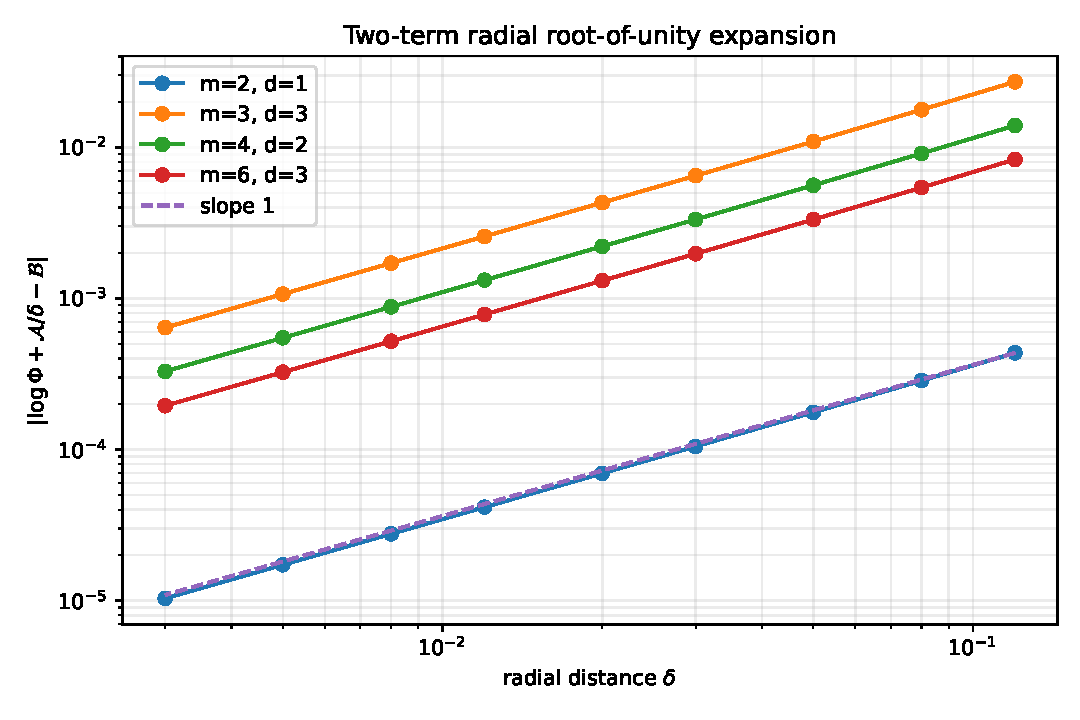
\includegraphics[width=0.91\textwidth]{radial_action_convergence.pdf}
 \caption{For $z=0.8$, the residual
 $|\log\Phi+\mathscr A/\delta-\mathscr B|$ is asymptotically linear in $\delta$ at four root orders.  The fitted slopes over the five smallest radial distances are all between $1.0043$ and $1.0045$.}
 \label{fig:radial}
\end{figure}

The calculation tests both the divergent action and the finite constant term.  It is notably sensitive to the $(2k-1)/(4k)$ term in \cref{eq:res-exp}; omitting that term changes the residual from $O(\delta)$ to $O(1)$.

\subsection{Blow-up and inverse errors}

\begin{figure}[H]
 \centering
 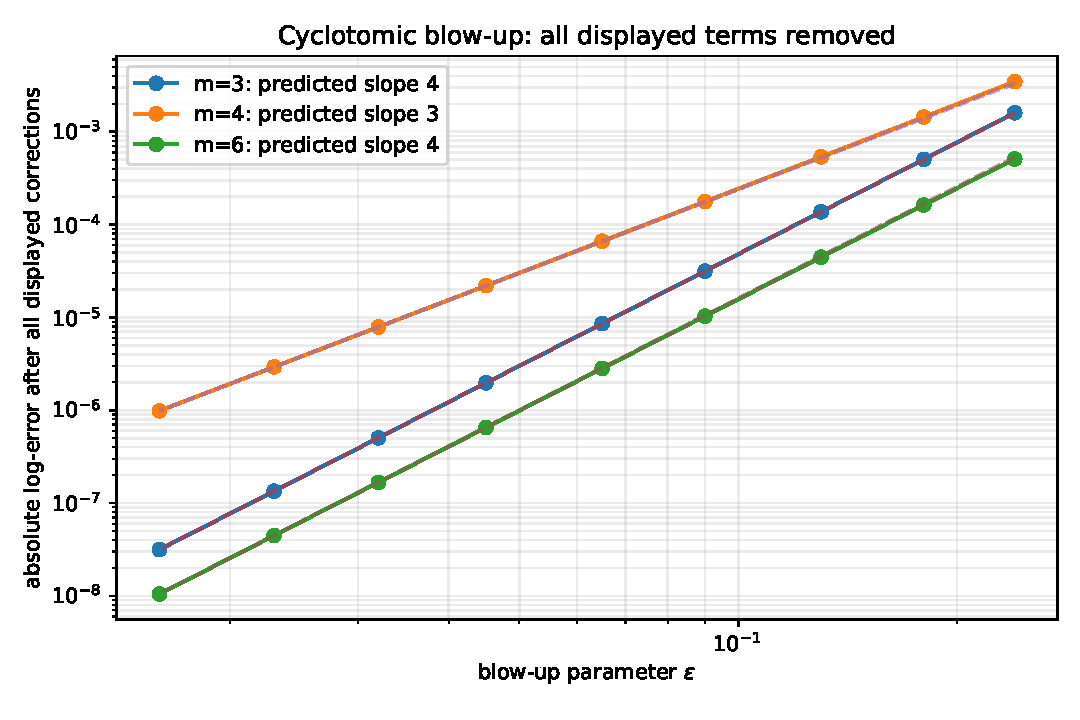
\includegraphics[width=0.91\textwidth]{cyclotomic_blowup_errors.pdf}
 \caption{Absolute logarithmic error after removing the limit, all subcritical terms, and the complete order-$\eps^d$ layer.  The predicted next exponents are $d+1$: four for $m=3,6$ and three for $m=4$.}
 \label{fig:blowup}
\end{figure}

\begin{figure}[H]
 \centering
 \begin{subfigure}{0.49\textwidth}
  \centering
  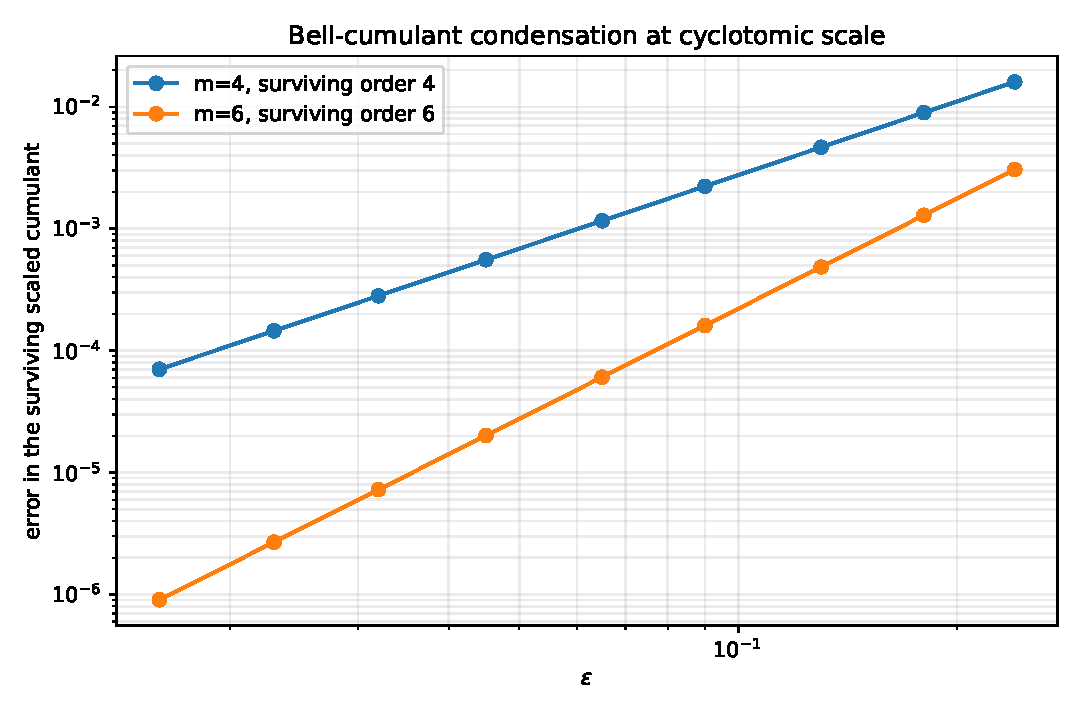
\includegraphics[width=\textwidth]{bell_moment_collapse.pdf}
  \caption{Surviving cumulant error.}
  \label{fig:bell}
 \end{subfigure}\hfill
 \begin{subfigure}{0.49\textwidth}
  \centering
  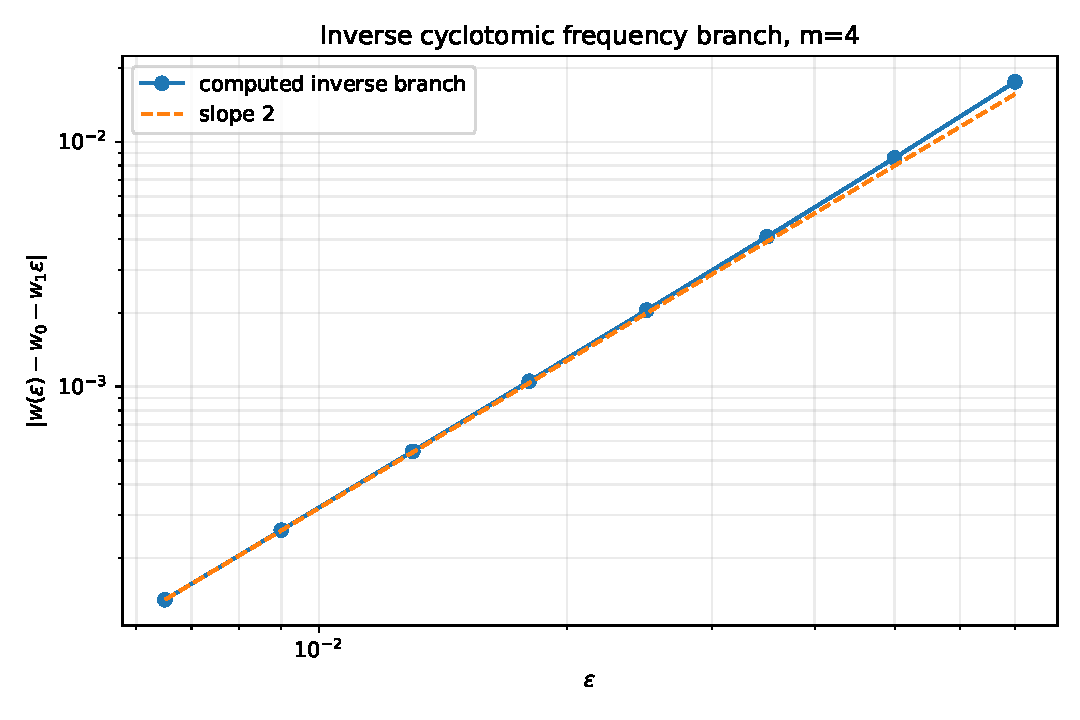
\includegraphics[width=\textwidth]{inverse_branch_errors.pdf}
  \caption{Inverse frequency error.}
  \label{fig:inverse}
 \end{subfigure}
 \caption{The Bernoulli cumulant converges to the unique order-$2d$ limit; the first-order inverse frequency formula has the predicted quadratic remainder.}
\end{figure}

\subsection{Fitted exponents}

\begin{table}[H]
 \centering
 \caption{Log--log slopes fitted to the five smallest parameters.  The final column gives the absolute error at the smallest tested parameter.}
 \label{tab:slopes}
 \begin{tabular}{@{}lrrr@{}}
\toprule
diagnostic & predicted slope & fitted slope & last error\\
\midrule
fixed radial, $m=2$ & 1 & 1.0043 & $1.034e-05$\\
fixed radial, $m=3$ & 1 & 1.0044 & $6.407e-04$\\
fixed radial, $m=4$ & 1 & 1.0044 & $3.289e-04$\\
fixed radial, $m=6$ & 1 & 1.0045 & $1.949e-04$\\
blow-up, $m=3$ & 4 & 4.0001 & $3.146e-08$\\
blow-up, $m=4$ & 3 & 3.0041 & $9.846e-07$\\
blow-up, $m=6$ & 4 & 3.9934 & $1.045e-08$\\
inverse frequency, $m=4$ & 2 & 2.0210 & $1.350e-04$\\
inverse $q$-branch, $m=4$ & 8 & 7.9960 & $3.534e-08$\\
\bottomrule
\end{tabular}

\end{table}

The inverse $q$ experiment at $\omega=\ImaginaryUnit$ fixes $y=1.1$ and solves for
\(q(z)=\ImaginaryUnit(1-\delta(z))\).  The leading approximation has error $O(z^6)$; after the $C_{1,\omega}$ correction, the fitted exponent is $7.9960$, matching the predicted $O(z^8)$ remainder.  At $z=0.145$, the exact radial coordinate was
\[
 \delta=2.57314407304007927\times10^{-5}
 +9.47348632511157983\times10^{-7}\ImaginaryUnit,
\]
while the two-term absolute error was $3.53\times10^{-8}$.

\begin{status}[Role of computation]
The numerical experiments do not substitute for the proofs.  They check constants, signs, and asymptotic orders, and they are especially useful for detecting missing resonant correction terms.  All theorem statements above are derived analytically from the locally uniformly convergent series.
\end{status}

\section{Connections with Thue--Morse and cyclic digital structure}

The original dyadic theory combines two kinds of scale symmetry.  The sinc product uses geometric scales $2^{-j}$, while the Thue--Morse polynomial
\(
 \prod_{j<N}(1-z^{2^j})
\)
encodes binary digit parity.  The cyclotomic analysis introduces a third viewpoint: a periodic character in the \emph{scale index} $j$.

At $q=\omega(1-\delta)$, the leading phases $q^j\approx\omega^j$ repeat with period $m$.  Because sinc is even, the logarithm sees $\omega^{2j}$ and the effective period is $d$.  The cyclic projector in \cref{eq:cyclic-projection} is precisely the finite Fourier projection onto the resonant scale characters.  At $\omega=-1$, the period-two character collapses to $d=1$ and produces the Gaussian limit.  Higher roots produce higher-order heat symbols.

This does not identify the cyclotomic scale character with the Thue--Morse sequence itself: Thue--Morse parity is generated by binary digits of the \emph{summation index}, whereas $\omega^j$ is periodic in the \emph{scale position}.  A promising bridge is to combine the two characters in a two-nome product, exactly the larger problem left open in the repository.

\begin{problem}[Thue--Morse/cyclotomic coupling]
For finite products carrying both a Thue--Morse sign and a scale phase $\omega^j$, determine the resonant cumulant order, the analogue of $\mathscr A_\omega$, and whether Prouhet cancellation can suppress the leading spectral dilogarithm.  Classify the resulting limit symbols by the joint character group.
\end{problem}

\section{Further conjectures and research directions}

\subsection{Maximal natural-boundary domain}

\begin{conjecture}[Natural boundary outside a discrete exceptional set]
For every fixed $z\ne0$ outside a locally finite exceptional set determined by simultaneous zeros of the actions $\mathscr A_\omega(z)$, the unit circle is a natural boundary for $q\mapsto\Phi(q,z)$.
\end{conjecture}

The theorem proved here covers $0<|z|<\pi/2$ uniformly.  Beyond that disk, the dilogarithm arguments cross branch cuts and the sign argument no longer applies.  A useful first target is to show that each $\mathscr A_\omega$ is not identically zero and has a discrete zero set; a Baire-category argument might then yield generic natural boundary, while arithmetic control of intersections could sharpen ``generic'' to an explicit complement.

\subsection{Cyclic quantum dilogarithm in the finite term}

The leading action is dilogarithmic, while standard root-of-unity asymptotics of $q$-Pochhammer symbols also contain a finite cyclic quantum dilogarithm.  Formula \cref{eq:B-first,eq:B-second} should admit a factorized form obtained by multiplying the cyclic factors over $n$ in \cref{eq:qpoch-factor}.

\begin{problem}[Spectral cyclic dilogarithm]
Find a convergent regularized product $\mathcal D_\omega(z)$ such that
\[
 \EulerE^{\mathscr B_\omega(z)}
 =\mathcal E_\omega(z)\mathcal D_\omega(z),
\]
where $\mathcal E_\omega$ is an elementary square-root factor and $\mathcal D_\omega$ is an infinite spectral product of finite cyclic quantum dilogarithms.  Determine its functional equations and zero divisor.
\end{problem}

\subsection{Irrational boundary phases and small divisors}

At an irrational point $q=\EulerE^{2\pi\ImaginaryUnit\alpha}$ there is no exact resonance, but denominators $1-q^{2k}$ can be arbitrarily small.  Diophantine properties of $\alpha$ should govern the boundary growth.

\begin{conjecture}[Diophantine phase transition]
For badly approximable $\alpha$, suitably Abel-regularized logarithms of $\Phi(r\EulerE^{2\pi\ImaginaryUnit\alpha},z)$ admit polynomial bounds as $r\uparrow1$ on a small frequency disk.  For Liouville $\alpha$, there exist frequency values with superpolynomial subsequential growth generated by near-resonant cumulants.
\end{conjecture}

This would interpolate between the exact root-of-unity action and generic natural-boundary behavior through small-divisor analysis.

\subsection{Arithmetic of the cyclotomic constants}

The constants
\[
 A_\omega=\frac{\zeta(2d)}{2d^2\pi^{2d}}(1-\omega)^{2d}
\]
are algebraic because $\zeta(2d)/\pi^{2d}$ is rational.  Their signs are elementary, but their Galois traces, norms, and divisibility encode nontrivial cyclotomic arithmetic.

\begin{problem}[Galois packets]
For fixed $m$, determine the trace and norm of $A_\omega$ over all primitive $m$th roots, and similarly for the correction coefficients $C_{k,\omega}$.  Relate their prime valuations to cyclotomic units and Bernoulli numerators.
\end{problem}

\subsection{Uniform double scaling in root order}

The present analysis fixes $m$.  When $m\to\infty$, the resonance order $d$ grows, $A_\omega$ becomes very small, and the limit exponent has increasing degree.  There should be a second asymptotic regime balancing $d$, $\eps$, and $w$.

\begin{problem}[Large-order cyclotomic saddle]
Determine a scaling in which
\(
 A_\omega w^{2d}
\)
remains nontrivial as $d\to\infty$, and identify whether the limiting profile is a hard cutoff, an extreme-value law, or a new Lambert-$W$ saddle.  Track the transition between polyharmonic kernels and the endpoint asymptotics already developed in the repository.
\end{problem}

\subsection{Inverse monodromy and branch braiding}

The $2d$ inverse frequency branches and the infinitely many logarithm sheets of $y$ form a branched covering.  The first coefficients are explicit, but global continuation may braid branches around zeros of $\Phi$.

\begin{conjecture}[Cyclotomic inverse braid]
For generic target $y$, continuation around a simple zero of the finite-level sinc product acts by a transposition on inverse branches, while continuation around $y=0$ acts by the cyclic rotation $w_0\mapsto\EulerE^{\pi\ImaginaryUnit/d}w_0$.  In the infinite limit these generators produce a nontrivial braid representation compatible with the escaping zero cloud.
\end{conjecture}

\subsection{Two-nome extension}

The repository's open problem asks for a two-nome phase diagram and canonical root-of-unity limits.  The scalar theorem suggests the correct first invariant: identify the lowest Taylor monomial whose bidegree resonates with the pair of roots.  The universal germ proof extends almost verbatim to
\[
 \prod_{j\ge0}h\bigl((1-\rho)\rho^jz,(1-\sigma)\sigma^jw\bigr),
\]
but the resonance set is now a lattice rather than a single arithmetic progression.  Its Newton polygon should determine the anisotropic scaling and the limiting exponential polynomial.

\begin{conjecture}[Newton-polygon resonance principle]
For an analytic two-variable germ, the canonical two-nome root-of-unity blow-up is determined by the lower convex hull of resonant Taylor exponents.  A single vertex gives a monomial exponential; an edge gives a genuinely multivariate exponential polynomial and a coupled polyharmonic PDE.
\end{conjecture}

\subsection{Formalization roadmap}

The new theory has a favorable dependency graph.
\begin{enumerate}[label=\arabic*.]
\item \textbf{Finite algebra.}  Formalize $d=\ord(\omega^2)$, the resonant/nonresonant split, and the exact first two coefficients of \cref{eq:res-exp}.
\item \textbf{Formal power series.}  Prove the coefficient identity \cref{eq:Ln} in a Laurent-series ring; Bell exponentiation is already well suited to existing combinatorial infrastructure.
\item \textbf{Finite cyclic projection.}  Prove
\(
 d^{-1}\sum_{r<d}\omega^{2kr}=\mathbf1_{d\mid k}
\)
and derive a finite-truncation version of \cref{eq:cyclic-projection}.
\item \textbf{Analytic tails.}  Establish geometric majorants for $|a_\omega z|<\pi$ and pass from truncations to the radial theorem.
\item \textbf{Sign and natural boundary.}  Formalize the sign of $a_\omega^{2d}$ and $\Polylogarithm_2(\pm x)$ on $0<x<1$, then use the finite-order zero/pole contradiction.
\item \textbf{Moments.}  Reuse the repository's Bernoulli cumulant and Bell moment APIs to prove the one-cumulant limit.
\item \textbf{Inverse branches.}  Begin with formal coefficient recursion; defer the analytic implicit-function theorem until the local complex-analysis library is convenient.
\end{enumerate}

A compact first formal milestone would prove the blow-up limit and sparse moment formula without dilogarithms.  The natural-boundary theorem can then be added after the sign representation is available.

\section{Conclusion}

The complex $q$-plane reveals a structure invisible on the positive real interval.  At every root of unity, the geometric sinc product organizes itself by the order of $\omega^2$.  Fixed frequencies see a spectral dilogarithmic action of size $1/\delta$; shrinking frequencies at the exact cyclotomic rate isolate one resonant coefficient and produce a pure exponential $\EulerE^{-A_\omega w^{2d}}$.  The same resonance appears simultaneously in the zero divisor, Bernoulli cumulants, Bell moments, and inverse Appell polynomials.

This unifies several themes of the Fabius--Rvachev corpus without duplicating its existing results.  The sinc product supplies the spectral side; $q$-Pochhammer factorization explains the dilogarithm; Bell and Bernoulli polynomials control corrections and moments; root order determines a polyharmonic PDE; inverse-function theory reveals branch geometry; and the density of roots of unity turns the local action into a global natural boundary.  The scalar root-of-unity renormalization is therefore not an isolated asymptotic trick but a common cyclotomic layer connecting the repository's $q$-analog, Fourier, moment, and inverse theories.

\appendix

\section{Uniformity details for the radial theorem}

Let $K\Subset\SetOf{z:|a_\omega z|<\pi}$ and choose $\rho<1$ such that
\(
 |a_\omega z|\le\rho\pi
\) on $K$.  The coefficient bound
\begin{equation}
 c_k|a_\omega z|^{2k}
 \le \frac{\zeta(2)}{k}\rho^{2k}
 \label{eq:ck-majorant}
\end{equation}
provides the basic summable majorant.  The nonresonant denominators at $\delta=0$ run through a finite set
\(
 \SetOf{1-\omega^{2r}:1\le r<d}
\), so they are uniformly separated from zero.  The $s$th Taylor coefficient in $\delta$ of either numerator or denominator quotient grows polynomially in $k$ for fixed $s$.  Therefore every fixed-order expansion is dominated by
\(
 C_s k^{M_s}\rho^{2k}
\), which is summable.  This proves not only \cref{eq:two-term-radial} but a full radial expansion
\begin{equation}
 \log\Phi(\omega(1-\delta),z)
 \sim -\frac{\Aact_\omega(z)}{\delta}
 +\sum_{r\ge0}B_{r,\omega}(z)\delta^r
 \label{eq:full-radial}
\end{equation}
locally uniformly in the same disk.  Each $B_{r,\omega}$ is an explicitly convergent zeta-weighted series with rational functions of $k$ and $\omega$ as coefficients.

\section{A direct coefficient derivation for the inverse $q$-branch}

Set
\(
 \delta=\rho z^{2d}
\).  The $k=d$ term in the logarithm is
\begin{align}
 -c_dz^{2d}
 \frac{(a_\omega+\omega\rho z^{2d})^{2d}}
 {1-(1-\rho z^{2d})^{2d}}
 &=-\frac{A_\omega}{\rho}
 +O(z^{2d}).
 \label{eq:rho-leading}
\end{align}
For $1\le k<d$, the nonresonant terms are
\begin{equation}
 -C_{k,\omega}z^{2k}+O(z^{2k+2d}).
 \label{eq:rho-nonres}
\end{equation}
Write
\begin{equation}
 \rho(z)=\rho_0+\rho_1z^2+O(z^4),
 \qquad
 \rho_0=-\frac{A_\omega}{\ell}.
 \label{eq:rho-series}
\end{equation}
Then
\[
 -\frac{A_\omega}{\rho(z)}
 =\ell+\ell\left(-\frac{\rho_1}{\rho_0}\right)z^2+O(z^4).
\]
Matching the $-C_{1,\omega}z^2$ term gives
\(
 \rho_1/\rho_0=-C_{1,\omega}/\ell
\), which is \cref{eq:delta-z}.  Higher coefficients follow triangularly because the derivative in $\rho$ never vanishes at $\rho_0$.

\section{Exact small-order constants}

\begin{table}[H]
\centering
\caption{Leading constants for selected primitive roots $\omega=\EulerE^{2\pi\ImaginaryUnit/m}$.}
\begin{tabular}{@{}ccccc@{}}
\toprule
$m$ & $d$ & $a_\omega^{2d}$ & $A_\omega$ & real-axis type\\
\midrule
$2$ & $1$ & $4$ & $1/3$ & dissipative Gaussian\\
$3$ & $3$ & $-27$ & $-1/630$ & backward sixth order\\
$4$ & $2$ & $-4$ & $-1/180$ & backward fourth order\\
$6$ & $3$ & $1$ & $1/17010$ & dissipative sixth order\\
\bottomrule
\end{tabular}
\end{table}

For general primitive order $m$, the sign rule is
\[
 A_\omega>0\iff m\equiv2\pmod4,
 \qquad
 A_\omega<0\iff m\text{ is odd or }4\mid m.
\]
The magnitude can be written
\begin{equation}
 |A_\omega|
 =\frac{\zeta(2d)}{2d^2\pi^{2d}}
 \left(2\sin\frac{\pi h}{m}\right)^{2d}.
 \label{eq:A-magnitude}
\end{equation}

\section{Reproducibility manifest}

The companion archive contains:
\begin{center}
\begin{tabularx}{0.96\textwidth}{@{}p{0.45\textwidth}X@{}}
\toprule
path & purpose\\
\midrule
\texttt{cyclotomic\_q\_fabius\_frontier.tex} & complete manuscript\\
\texttt{cyclotomic\_q\_fabius\_frontier.pdf} & compiled and visually inspected PDF\\
\texttt{numerical\_experiments.py} & commented high-precision experiments\\
\texttt{data/*.csv} & raw deterministic numerical tables\\
\texttt{data/experiment\_summary.txt} & concise diagnostic output\\
\texttt{figures/*.pdf, figures/*.png} & vector and raster figures\\
\texttt{corpus\_audit\_note.txt} & audit method and novelty boundary\\
\texttt{corpus\_inventory\_2026-08-27.txt} & preserved 57-path recursive ledger\\
\texttt{requirements.txt} & Python dependencies\\
\texttt{README.txt} & build and reproduction instructions\\
\bottomrule
\end{tabularx}
\end{center}

The script uses the exact convergent logarithmic series rather than a truncated product.  To reproduce the tables and figures, run
\begin{lstlisting}[style=py]
python numerical_experiments.py --dps 80
\end{lstlisting}
from the archive root.  The LaTeX source expects the generated figure and data directories in their packaged relative locations.

\begin{thebibliography}{99}

\bibitem{ProveItDocs}
V.~Reshetnikov,
\newblock \emph{ProveIt: Analysis/FabiusFunction documentation corpus},
\newblock GitHub repository, living tree and archive,
\newblock \url{https://github.com/VladimirReshetnikov/ProveIt/tree/main/Analysis/FabiusFunction/docs},
accessed 30 August 2026.

\bibitem{ProveItPrimary}
V.~Reshetnikov,
\newblock \emph{The Fabius Function and Rvachev's Up-Function},
\newblock primary exposition in the ProveIt repository, 2026.

\bibitem{ProveItQFrontiers}
V.~Reshetnikov,
\newblock \emph{Exponents and $q$-Series Frontiers},
\newblock consolidated semi-formalized source in
\path{Analysis/FabiusFunction/docs/semi-formalized-research-frontiers/drafts/exponents-and-q-series}, 2026.

\bibitem{Fabius1966}
J.~Fabius,
\newblock A probabilistic example of a nowhere analytic $C^\infty$-function,
\newblock \emph{Zeitschrift f\"ur Wahrscheinlichkeitstheorie und Verwandte Gebiete}
\textbf{5} (1966), 173--174.

\bibitem{Rvachev1971}
V.~L.~Rvachev and V.~A.~Rvachev,
\newblock A certain finite function,
\newblock \emph{Dopovidi Akademii Nauk Ukrains'koi RSR, Series A} (1971), 705--707, 764.

\bibitem{Rvachev1990}
V.~A.~Rvachev,
\newblock Compactly supported solutions of functional-differential equations and their applications,
\newblock \emph{Russian Mathematical Surveys} \textbf{45} (1990), no.~1, 87--120.

\bibitem{Arias1982}
J.~Arias de Reyna,
\newblock An infinitely differentiable function with compact support: definition and properties,
\newblock English translation, arXiv:1702.05442.

\bibitem{AriasArithmetic}
J.~Arias de Reyna,
\newblock Arithmetic of the Fabius function,
\newblock \emph{INTEGERS} \textbf{18} (2018), Article A51; arXiv:1702.06487.

\bibitem{AlloucheShallit}
J.-P.~Allouche and J.~Shallit,
\newblock \emph{Automatic Sequences: Theory, Applications, Generalizations},
\newblock Cambridge University Press, 2003.

\bibitem{GasperRahman}
G.~Gasper and M.~Rahman,
\newblock \emph{Basic Hypergeometric Series}, second edition,
\newblock Cambridge University Press, 2004.

\bibitem{McIntosh1999}
R.~J.~McIntosh,
\newblock Some asymptotic formulae for $q$-shifted factorials,
\newblock \emph{Ramanujan Journal} \textbf{3} (1999), 205--214.

\bibitem{GaroufalidisZagier}
S.~Garoufalidis and D.~Zagier,
\newblock Asymptotics of Nahm sums at roots of unity,
\newblock \emph{Ramanujan Journal} \textbf{55} (2021), 219--238.

\bibitem{Kopp}
G.~S.~Kopp,
\newblock The Shintani--Faddeev modular cocycle,
\newblock preprint, 2024; sections on cyclic quantum dilogarithms and root-of-unity $q$-Pochhammer asymptotics.

\bibitem{BellComtet}
L.~Comtet,
\newblock \emph{Advanced Combinatorics},
\newblock Reidel, 1974.

\bibitem{EvgrafovPostnikov}
M.~A.~Evgrafov and M.~M.~Postnikov,
\newblock Asymptotic behavior of Green's functions for parabolic and elliptic equations with constant coefficients,
\newblock \emph{Mathematics of the USSR-Sbornik} \textbf{11} (1970), 1--24.

\end{thebibliography}

\end{document}
